\apendice{Especificación de Requisitos}

\section{Introducción}
En este apartado se especificarán las necesidades funcionales que se pretende alcanzar. Para ello se describirán los requisitos del software que se quiere desarrollar.

\section{Objetivos generales}
\begin{itemize}
    \item Como ya de describió en la memoria, el objetivo del proyecto es diseñar y desarrollar un videojuego de tipo «arcade». Para la implementación del juego que sirve como base para este proyecto, es necesario planear las mecánicas de juego, además de diseñar los modelos del jugador, los enemigos y otros elementos gráficos. Esta tarea también incluye el diseño de la interfaz, banda sonora y efectos de sonido. 
    
    \item Diseñar e implementar un sistema inteligente que posteriormente será utilizado para interactuar con el videojuego creado. Este proceso de divide en:
    \begin{itemize}
        \item Establecer una comunicación entre el juego y el modelo del sistema inteligente. Dado que el juego y el script que hace uso del modelo serán implementados en diferente lenguaje de programación, se debe establecer un mecanismo de intercambio de datos para la comunicación.
        \item Diseñar el conjunto de datos que posteriormente servirá para el entrenamiento del modelo. Al ser el punto de partida el aprendizaje por imitación, necesitaremos un gran volumen de datos de los cuales seleccionaremos todos o solo los más representativos para el entrenamiento.
        \item Implementar, haciendo uso de las bibliotecas como scikit-learn (minería de datos), DEAP(algoritmos evolutivos) y Pandas y NumPy (procesamiento de datos a bajo nivel) el sistema inteligente que jugará al videojuego.
    \end{itemize}
\end{itemize}

\section{Catalogo de requisitos}

\subsection{Especificación de requisitos}

\subsection{Requisitos funcionales}
Los requisitos funcionales que detallaré a continuación son so requisitos iniciales, ya que a lo largo del desarrollo, alguno de ellos se ve afectado por nuevas necesidades.

Los requisitos principales son:
\begin{itemize}
    \item RF1: Jugar al juego.
    \item RF2: Entrenar el modelo.
        \begin{itemize}
            \item RF2.1: Entrenar utilizando un Decision Tree
            \item RF2.2: Entrenar utilizando un Random Forest
            \item RF2.3: Entrenar utilizando un algoritmo evolutivo
        \end{itemize}
    \itme RF3: Explotar el modelo
        \begin{itemize}
            \item RF3.1: Explotar utilizando el modelo Decision Tree
            \item RF3.2: Explotar utilizando el modelo Random Forest
            \item RF3.3: Explotar utilizando el modelo algoritmo evolutivo
        \end{itemize}
\end{itemize}


\begin{figure}[h!]
    \centering
    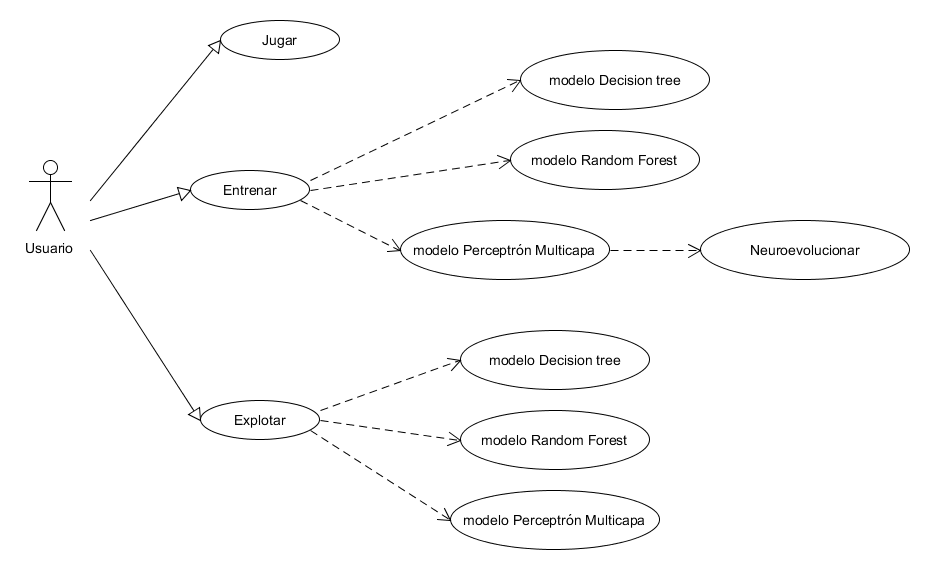
\includegraphics[width=0.6\textwidth]{casos_de_uso}
    \caption{Casos de uso}
    \label{fig:cuso}
\end{figure}




A continuación se procede a analiza en profundidad el RF1:
\begin{itemize}
    \item RF-1.1: Permitir que el jugador interactúe con la nave espacial, haciendo que se traslade lateralmente \ref{RF1}.
    \item RF-1.2: Permitir que el jugador pueda disparar \ref{RF2}.
    \item RF-1.3: Permitir que el jugador interactúe con el menú principal. El menú principal tiene dos botones \ref{RF3}.
        \begin{itemize}
            \item RF-1.3.1: El botón jugar lleva directamente a una nueva partida.
            \item RF-1.3.2: El botón salir permite salir del juego.
        \end{itemize}
    \item RF-1.4: El juego debe tener la capacidad de escribir los estados en un fichero \ref{RF4}.
\end{itemize}



\begin{table}[h!]
\centering
\begin{tabular}{|l|l|}
\hline
\multicolumn{2}{|l|}{\cellcolor[HTML]{C0C0C0}R1.1: Permitir que el jugador interactúe con la nave espacial}                                                           \\ \hline
Versión         & 1.0                                                                                                                                               \\ \hline
Autor           & Pablo Alejos                                                                                                                           \\ \hline
Descripción     & \begin{tabular}[c]{@{}l@{}}El jugador debe ser capaz de controlar la nave espacial haciendo\\ uso de las teclas izquierda y derecha.\end{tabular} \\ \hline
Precondiciones  & El jugador debe estar vivo, y la partida activa                                                                                                   \\ \hline
Acciones        & El usuario pulsa las teclas izquierda y derecha para controlar la nave.                                                                           \\ \hline
Postcondiciones & \begin{tabular}[c]{@{}l@{}}La nueva posición del jugador no podrá ser la misma que antes de pulsar\\ los controles.\end{tabular}                  \\ \hline
Excepciones     & \begin{tabular}[c]{@{}l@{}}Una pared puede bloquear el movimiento, por lo que la posición seguirá\\ siendo la misma\end{tabular}                  \\ \hline
Importancia     & Muy alta                                                                                                                                          \\ \hline
\end{tabular}
\caption{RF-1: Permitir que el jugador interactúe con la nave espacial}
\label{RF1}
\end{table}


\begin{table}[h!]
\centering
\begin{tabular}{|l|l|}
\hline
\multicolumn{2}{|l|}{\cellcolor[HTML]{C0C0C0}R1.2 Permitir que el jugador pueda disparar.}                                                                    \\ \hline
Versión         & 1.0                                                                                                                                       \\ \hline
Autor           & Pablo Alejos                                                                                                                    \\ \hline
Descripción     & El jugador debe ser capaz de disparar pulsando la tecla espaciadora.                                                                      \\ \hline
Precondiciones  & \begin{tabular}[c]{@{}l@{}}El arma tiene una cadencia, tiene que pasar un tiempo determinado para\\ poder volver a disparar.\end{tabular} \\ \hline
Acciones        & El usuario pulsa la tecla de disparo (Barra espaciadora).                                                                                 \\ \hline
Postcondiciones & Se debe producir un único dispatro.                                                                                                       \\ \hline
Excepciones     & \begin{tabular}[c]{@{}l@{}}Si no ha pasado el tiempo necesario desde el ultimo disparo no debe\\ disparar\end{tabular}                    \\ \hline
Importancia     & Alta                                                                                                                                      \\ \hline
\end{tabular}
\caption{RF-2: Permitir que el jugador pueda disparar.}
\label{RF2}
\end{table}


\begin{table}[h!]
\centering
\begin{tabular}{|l|l|}
\hline
\multicolumn{2}{|l|}{\cellcolor[HTML]{C0C0C0}RF-3: Permitir que el jugador interactúe con el menú principal.} \\ \hline
Versión                                   & 1.0                                                               \\ \hline
Autor                                     & Pablo Alejos Salamanca                                            \\ \hline
Descripción                               & El jugador interactúa con el menú principal                       \\ \hline
Precondiciones                            & -                                                                 \\ \hline
                                          & RF-3.1: el jugador pulsa empezar partida                          \\ \cline{2-2} 
\multirow{-2}{*}{Acciones}                & RF-3.2: el jugador pulsa el botón salir                           \\ \hline
                                          & RF-3.1: cambia de escena, pasando a la pantalla de juego.         \\ \cline{2-2} 
\multirow{-2}{*}{Postcondiciones}         & RF-3.2: sale de juego.                                            \\ \hline
Excepciones                               & No tiene.                                                         \\ \hline
Importancia                               & Alta                                                              \\ \hline
\end{tabular}
\caption{RF-3: Permitir que el jugador interactúe con el menú principal}
\label{RF3}
\end{table}


\begin{table}[h!]
\centering
\begin{tabular}{|l|l|}
\hline
\multicolumn{2}{|l|}{\cellcolor[HTML]{C0C0C0}RF-4: El juego debe tener la capacidad de escribir los estados en un fichero.}                                                                                               \\ \hline
Versión         & 1.0                                                                                                                                                                                                     \\ \hline
Autor           & Pablo Alejos Salamanca                                                                                                                                                                                  \\ \hline
Descripción     & \begin{tabular}[c]{@{}l@{}}A lo largo de la partida el juego debe registrar tanto el\\ estado de la partida como las acciones del jugador. Estas\\ instancias de graban en un fichero csv.\end{tabular} \\ \hline
Precondiciones  & Tiene que haber una partida activa que poder grabar.                                                                                                                                                    \\ \hline
Acciones        & El jugador hace uso del juego para generar el fichero.                                                                                                                                                  \\ \hline
Postcondiciones & \begin{tabular}[c]{@{}l@{}}Cuando acaba la partida debe existir un fichero denominado\\ gamestates\_XX.csv\end{tabular}                                                                                 \\ \hline
Excepciones     & -                                                                                                                                                                                                       \\ \hline
Importancia     & Alta                                                                                                                                                                                                    \\ \hline
\end{tabular}
\caption{RF-4: El juego debe tener la capacidad de escribir los estados en un fichero.}
\label{RF4}
\end{table}